\chapter{Application to manual wheelchair locomotion}
\section{Introduction}
To improve the efficiency of wheelchair propulsion, a Wheelchair Ergometer (FRET-2) equipped with sensors has been manufactured. The sensors installed on the wheelchair measure the physical stresses applied to the Manual Wheelchair (FRM) during actual use and record them. The following paragraphs present.
\begin{itemize}
\item A description of the measurements recorded by the sensors during actual use;
\item An analysis of the data obtained by applying  the algorithms as mentioned above (in our contribution).
\end{itemize}

\begin{flushright}

\end{flushright}
\section{Description of the dataset}

\begin{figure}[h]
\center
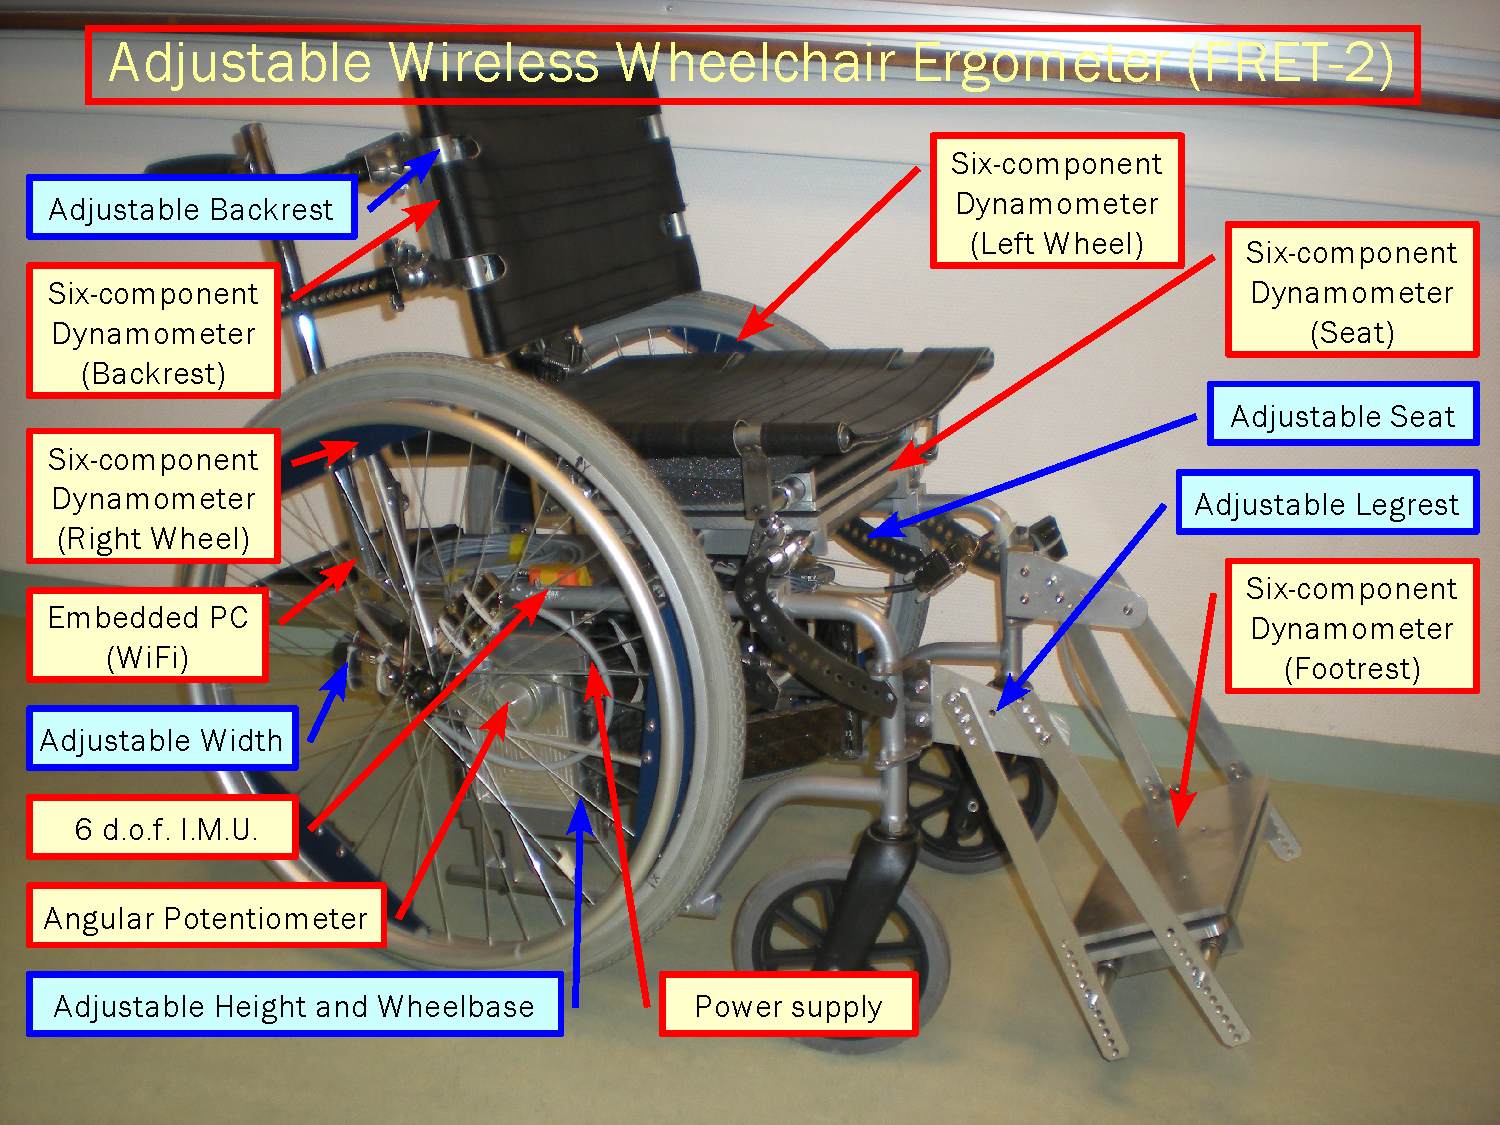
\includegraphics[scale = 0.4]{images/FRET-2_Legend_GB}
\caption{title}
\label{fret_legend}
\end{figure}


The sensors are located on the right and left wheels of the manual wheelchair, on the footrest, on the seat and the backrest (see Figure \ref{fret_legend}). These sensors measure the forces and moments of these forces applied to each of the systems mentioned above.  The moment of a force concerning a given point is a vectorial physical quantity which translates the ability of a force to turn a mechanical system around that point, often called a pivot [20]. The sensors installed on the FRM were used to measure the kinematic parameters (speed, acceleration) of the movement of the Manual Wheelchair (FRM), as well as its position relative to the Earth's magnetic north.

The measurements recorded by the sensors and subjected to our analysis consist of 44 attributes; 30 of the 44 attributes relate to the measurement of the torque constituted by force applied to the systems mentioned above and the moment of this force to an axis of rotation. For each of the five systems, we have three components of the force (Fx, Fy, Fz) and the momentum (Mx, My, Mz) that apply to it. The 14 other attributes tell us about the kinematics of the manual wheelchair and its position relative to the Earth's magnetic north. The detailed description of these data is presented in Table 4.1.

To analyze the propulsion in FRM, we are interested in the moment along the axis of Z (Mz) applied to the right and left wheels of the FRM. This will allow us to identify the propulsion cycles during the move. A propulsion cycle consists of a push time interval and a consecutive freewheeling time interval that materializes on the Z-moment by a peak and drag as shown in Figure 4.2. The description of the data recorded by the sensors is presented in Appendix B.

\subsection{Torque sensor}
\subsection{Characteristic properties of the data}
\subsubsection{The length}
\subsubsection{The cycles}
\subsubsection{The uncertainty}
\section{Analysis based on propulsion technique}
\section{Analysis based on propulsion capabilities}
\section{Propulsion technique versus propulsion capabilities}
\section{Conclusion}


